El filtro umbralizar consiste en evaluar cada pixel de la imagen y asignarle un nuevo valor según tres criterio.
\begin{itemize}
\item Si el pixel supera el máximo pasado por parámetro a la función, se le coloca un 255.
\item Si el pixel es menor que el mínimo, también pasado por parámetro, se le coloca un 0.
\item Si el pixel está entre ($min \leq pixel \leq max$), se le asigna $\lfloor pixel/q \rfloor * q$, donde q es un parámetro.
\end{itemize}

\subsubsection{Descripción del ciclo}
El filtro se divide en cinco etapas:
\begin{enumerate}
\item \textbf{Pre-ciclo:} Se crean ciertos registros que serán de utilidad en el ciclo.
\item \textbf{Inicio del ciclo:} Puesta en 0 del registro acumulador y obtención de máscara de mínimos.
\item \textbf{Obtención de la máscara para pixeles mayores al máximo y aplicación:} Se consigue la máscara para los pixeles que superen al mayor y se aplica al acumulador.
\item \textbf{Creación de la máscara para los pixeles ($min \leq pixel \leq max$):} Se arma la máscara a partir de una nueva comparación y máscaras anteriores.
\item \textbf{Aplicación de la máscara para ($min \leq pixel \leq max$) y fin del ciclo:} Se realizan los cálculos pertinentes a los pixeles que entran en esta categoría y lo aplica a la máscara.
\end{enumerate}

\subsubsection{Pre-ciclo}
Para optimizar el procesamiento dentro del ciclo, se calcula y se guarda en registros xmm al inicio del programa:
\begin{itemize}
  \item xmm12 $\Rightarrow$ Contiene 16 bytes packed con el mínimo
  \item xmm11 $\Rightarrow$ Contiene el mínimo packed en words
  \item xmm5 $\Rightarrow$ Contiene el máximo packed en words
  \item xmm6 $\Rightarrow$ Contiene la representación flotante de Q packed
\end{itemize}

También se calcula y se guarda en el registro rcx, la cantidad de pixeles que tiene la imagen, información que se utilizará para conocer cuántos pixeles faltan por procesar en cada iteración.

\subsubsection{Inicio del ciclo}
Al comienzo del ciclo se ponen en 0 los bytes del registro xmm8 que servirá como acumulador de los nuevos valores que tendrán los pixeles.

Se leen 16 bytes contiguos desde la imagen fuente en el registro xmm1 utilizando la instrucción movdqu, se busca cuáles son iguales al mínimo (aprovechando la instrucción pcmpeqb que realiza la comparación en los 16 bytes simultaneamente) y se guarda la máscara obtenida que se usará mas tarde.

\subsubsection{Obtención de la máscara para pixeles mayores al máximo y aplicación}

Queriendo explotar al máximo las instrucciones SIMD, tratando de procesar en simultaneo 16 bytes, encontramos que esto no era posible debido a que el set de instrucciones no contempla comparaciones de greater, lower o derivadas para bytes sin signo (necesario ya que los pixeles en grayscale van del 0 al 255), por lo que fue necesario extender los bytes mediante un desempaquetado, convirtiendolos en words, para luego hacer las comparaciones correspondientes.

\begin{figure}[H]
\centering
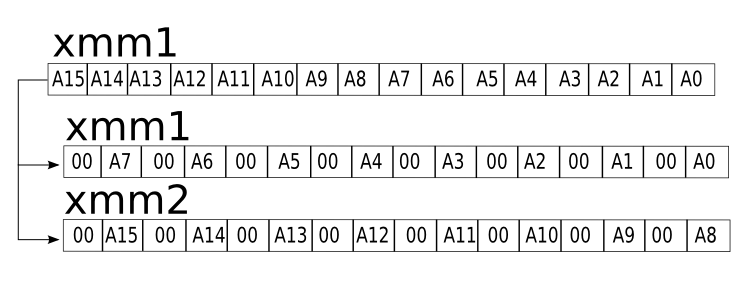
\includegraphics[width=90mm]{unpackxmm1.png}
\caption{Desempaquetado de los bytes a words para realizar comparaciones}
\label{overflow}
\end{figure}
Se desempaquetan los 16 bytes en parte baja (primeros 8 bytes) y en parte alta convirtiendolos a words por medio de la instrucción punpcklbw.

Se buscan los números que superen al máximo comparando la parte alta y baja con el registro xmm5 preparado al inicio del programa, el cuál contiene el máximo en words empaquetadas. Utilizando pcmpgtw tanto en la parte baja como la alta, obtenemos una máscara que contiene en 0xFFFF las words mayores al máximo y en 0x0000 las demás. Empaquetamos, utilizando la instrucción packsswb, la máscara relacionada a la parte baja y a la alta, dejando en 255 sólo los bytes que sean mayores al máximo para luego sumarlos en el acumulador utilizando paddusb.

\begin{figure}[H]
\centering
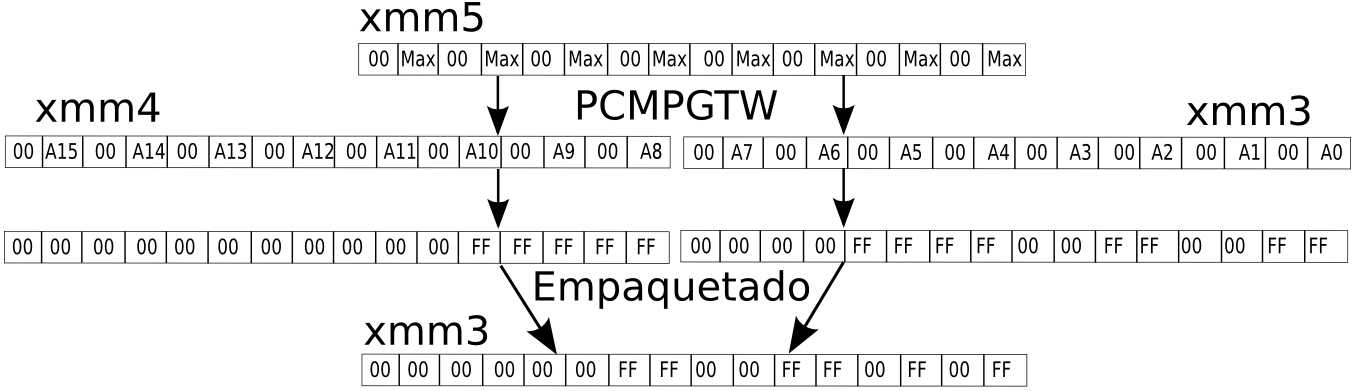
\includegraphics[width=150mm, height=40mm]{cpmmax.png}
\caption{Ejemplo de creación de máscara y empaquetado de la misma. El registro xmm3 es la copia de xmm1 que guardará la parte baja de la máscara, xmm4 realiza lo mismo con la parte alta.}
\label{overflow}
\end{figure}

\subsubsection{Creación de la máscara para los pixeles ($min \leq pixel \leq max$)}
Al utilizar un acumulador incialmente en 0 se pudo ahorrar el paso de comparar los pixeles menores al mínimo ya que los pixeles que cumplieran esta propiedad tendrían 0 como valor.

Para conseguir la máscara, se aprovechó las máscaras previamente obtenidas (mayores al máximo e iguales al mínimo), por lo que sólo fue necesario buscar los números mayores al mínimo (haciendo un procedimiento similar al de la búsqueda del máximo), agregarle los números iguales al mínimo (mediante un por) con la máscara creada al principio del ciclo y luego sacarle los mayores al máximo (mediante un pxor) dejandome sólo los pixeles que cumplen esta condición.

\subsubsection{Aplicación de la máscara para ($min \leq pixel \leq max$) y fin del ciclo}
Al ser necesaria un división y un truncamiento para el caso, se utilizaron single precision floats.

Fue necesario desempaquetar aún más los pixeles, utilizando punpcklwd, para poder obtener los valores de estos en double words, y poder convertirlos a single precision floats mediante la instrucción cvtdq2ps. Esta es precisión suficiente para los cálculos y además brinda la posibilidad realizar más operaciones sobre los pixeles simultanteamente que con doubles.

Se realiza el desempaquetado de la parte baja anteriormente desempaquetada (xmm1) y se los convierte a single presicion floats. Luego se los divide, utilizando divps, por el registro xmm6 el cuál contiene el valor Q empaquetado en single presicion floats calculado al inicio del programa. Se lo trunca utilizando cvttps2dq, para realizar la función floor ($\lfloor \rfloor$) convirtiendose en entero, se lo convierte otra vez a float y se lo termina multiplicando, utilizando mulps, por xmm6 otra vez para finalmente ser convertido a entero, obteniendo el valor correspondiente para cáda pixel. Se vuelve a empaquetar, utilizando la instrucción packusdw, obteniendose otra vez los valores nuevos de los pixeles en words y se repite la operación con la parte alta del desempaquetado inicial (xmm2).

\begin{figure}[H]
\centering
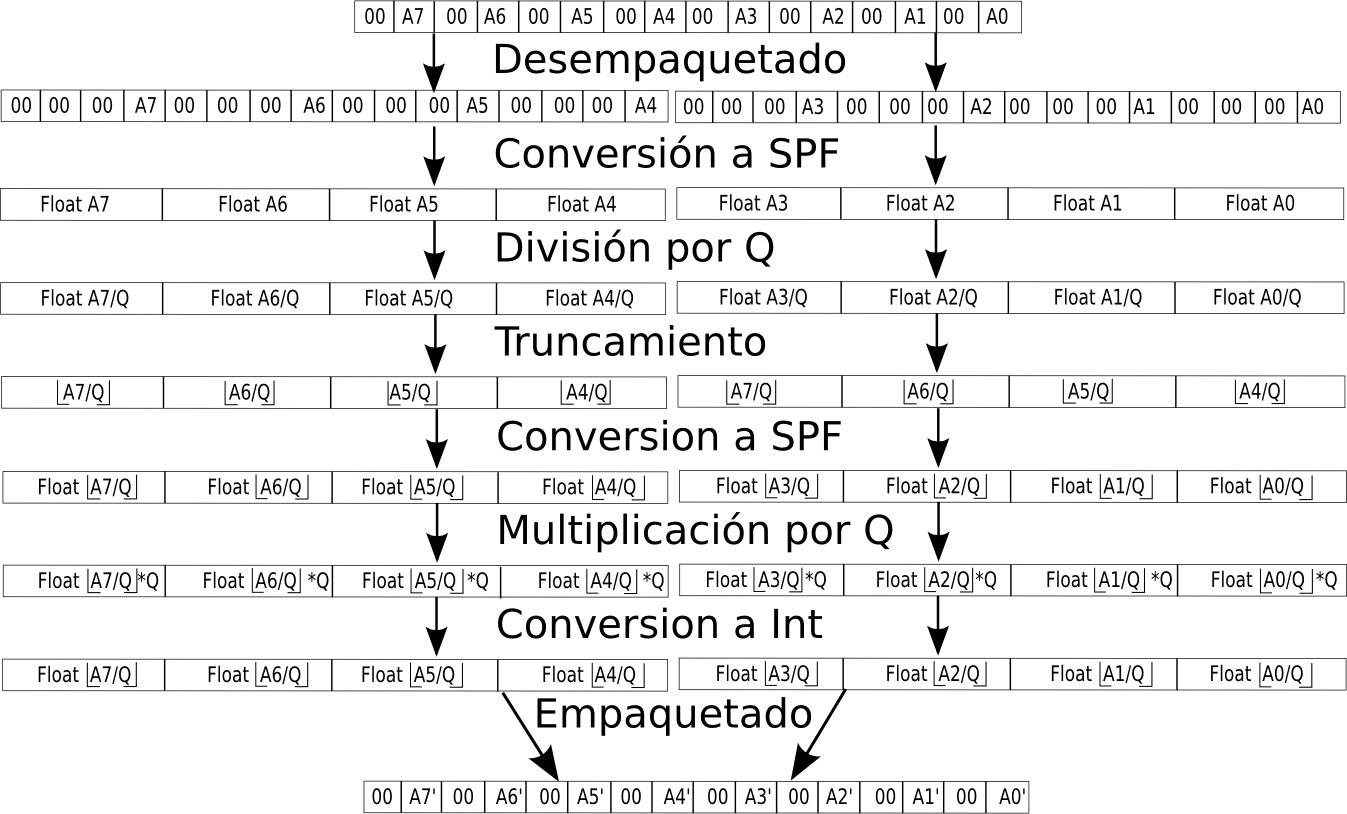
\includegraphics[width=150mm, height=85mm]{calcq.png}
\caption{Ejemplo del cálculo de la parte baja de los nuevos valores para los pixeles que entran en el caso ($min \leq pixel \leq max$), el mismo procedimiento se realiza con la parte alta y se empaquetan ambos resultados}
\label{overflow}
\end{figure}

Al finalizar, se empaquetan los dos registros resultantes, mediante packuswb, para luego poder aplicarle la máscara anteriormente creada para el caso utilizando un pand y sumar simultaneamente con paddusb el valor obtenido al acumulador, dejando el valor correspondiente en los pixeles que cumplían con el caso.

Por último, se copian los nuevos valores de los 16 bytes en la imagen destino utilizando movdqu y se incrementan los punteros de la imágen fuente y destino para la próxima iteración. También se resta nuestro contador de pixeles por procesar, se lo compara para ver si llegó al final, caso en el que termina la ejecución, o si quedan más e igual, caso en el que vuelve a ciclar, o si restan menos de 16 bytes por agarrar, dónde se vuelve para atrás los punteros de las imágenes para que queden 16 pixeles exactamente y se pueda realizar la última iteración.

\subsubsection{Comparación con la implementación C}
El ciclo en C hace escencialmente lo mismo que la implementación en assembler, pero esta lo hace de manera simultanea utilizando SIMD. 

Estos son los detalles de las operaciones realizadas en C para 16 bytes:
\begin{itemize}
\item 16 accesos a memoria para la lectura de cada byte y 16 para la escritura
\item Se realizan a lo sumo 32 comparaciones, (2 por cáda pixel), en dónde se necesita calcular la posición del pixel cáda vez que se lo quiere leer y se realiza un acceso a memoria para esto.
\item En caso de haber caído dentro del caso ($min \leq pixel \leq max$), se realizan cáda una de las operaciones de cálculo de manera secuencial.
\end{itemize}
Detalles de las operaciones realizadas por la implementación de assembler en 16 bytes:
\begin{itemize}
\item Única lectura y escritura en memoria de 16 bytes
\item Se realizan 2 comparaciones para el caso de los pixeles mayores al máximo y para calcular los píxeles mayores al mínimo por cada 16 bytes, ya que se comparan de a 8 bytes simultaneamente utilizando SIMD. También se realiza 1 comparación cada estos 16 bytes para obtener los iguales al mínimo.
\item Si bien siempre se realiza el cálculo en punto flotante relacionado a los valores de los pixeles del caso ($min \leq pixel \leq max$), estos se realizan con 4 instrucciones SIMD, pudiendo calcular el valor de 16 bytes por ciclo.
\end{itemize}

\subsubsection{Rendimiento}
Observamos las siguientes cantidades de ciclos y ticks de reloj al realizar 100 iteraciones de ambas implementaciones con una imagen cuadrada de lado 512 y utilando los parámetros: mín = 64, máx = 128 y Q = 16.
\begin{center}
    \begin{tabular}{|l|l|l|l|}
        \hline
        Medición & Implementación C & Implementación assembler & Relación \\
        \hline
        Ticks    & 785867600      & 70172072               & $8.92\%$ \\
        Ciclos   & 7858676        & 701721                & $8.92\%$ \\
        \hline
    \end{tabular}
\end{center}

Para hacer un análisis fino, utilizamos la herramienta objdump (objdump -d -M intel -S umbralizar\_c.o) para obtener el resultado de la compilación mediante gcc.

Destacamos de este análisis el uso contínuo de variables locales (almacenadas en el stack) y el cálculo de la posición en memoria y el acceso a esta cáda vez que se quería realizar una comparación, algo evitable usando registros en ensamblador y que seguro impactaron en la performance.

\begin{verbatim}
if(src_matrix[y][x] < min) {
;Instrucciones para settear la posicion del byte
mov    eax,DWORD PTR [rbp-0x4c]
movsxd rdx,eax
movsxd rax,ebx
imul   rdx,rax
mov    rax,QWORD PTR [rbp-0x38]
add    rdx,rax
mov    eax,DWORD PTR [rbp-0x48]
cdqe   
movzx  eax,BYTE PTR [rdx+rax*1]
;Termina el setteado de la posicion del byte
cmp    al,BYTE PTR [rbp-0x70] ;Realiza la comparacion
jae    c3 <umbralizar_c+0xc3>
\end{verbatim}

Cabe destacar que el lenguaje ensamblador, además del uso de las instrucciones SIMD, que nos permiten realizar cálculos simultaneamente otorgandonos una gran ventaja contra el código en C, también nos permite explotar los recursos al máximo, pudiendo obviar cálculos de más guardandolos para su posterior uso y utilizar registros que implican menos cantidad de accesos a memoria.

Estas ventajas, sumadas a los pocos accesos de memoria al poder escribir y leer de a 16 bytes son la causa del bajo tiempo de ejecución del filtro en ASM.